\chapter{History View}
\label{sec:history}

glscopeclient has the ability to save every waveform during a session in memory, allowing you to go back in time and
see previous state of the system being debugged. Clicking on a timestamp in the history view pauses acquisition and
loads the historical waveform data for analysis.

By default, the history view (Fig. \ref{historyview}) is not displayed and no history is captured. If the history view
is closed, history continues to be captured up to the configured maximum history depth.

\begin{figure}[H]
\centering
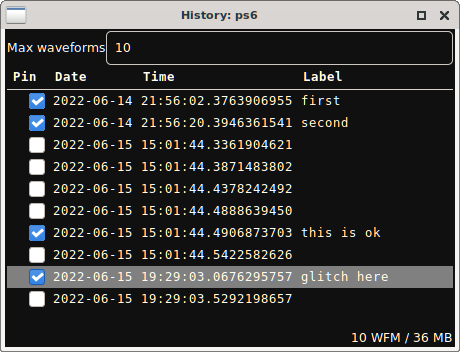
\includegraphics[width=5cm]{images/history-view.png}
\caption{Waveform history view}
\label{historyview}
\end{figure}

The ``max waveforms" box allows the depth of the history to be configured. It defaults to 10 but can be set to any
positive integer value. Older waveforms beyond the history limit are deleted as new waveforms are acquired.

The status bar at the bottom of the history view displays the total number of waveforms in the history, as well as an
estimate of the amount of RAM used by the history.

\section{Estimating Waveform Memory Usage}

When selecting a maximum depth for the history, it is important to pick a reasonable limit to avoid running out of RAM!
glscopeclient will happily fill tens or hundreds of gigabytes of memory with deep waveforms if given a chance. Memory
usage of waveform data can be roughly estimated as 16 + sizeof(sample type) bytes per point, since each sample contains a
64-bit timestamp and duration plus the sample data.

For example, an analog sample takes 20 bytes of RAM (16 of time plus a 32-bit floating point voltage measurement) per
sample. Thus, a 1M point analog waveform takes approximately 20 MB of RAM per channel, or 80 MB per capture on a
four-channel oscilloscope with all channels enabled.

On the larger side, a 10M point four channel capture would use 800 MB and a 64M point deep-memory capture would use 5
GB. A deep history setting, such as 100 waveforms, is thus wildly inappropriate for such deep captures! A future
software release may support spilling waveform data to a temporary directory on disk, permitting effectively unlimited
history depth given sufficient disk space.

Digital waveforms use one byte per sample for the actual measurement, so 17 MB per channel for a 1M point waveform.

Filter memory usage varies depending on the specific fitler in question, however it is typically not a large
contributor to the overall glscopeclient RAM footprint when using history mode because filters are evaluated
dynamically each time a waveform is pulled from history rather than having output cached for every historical waveform.
Thus, at most one copy of each filter's output is present in memory regardless of history depth.
